\vspace{0.8cm}

\section{Metodología}

\subsection{Limitaciones del entorno de simulación}

Durante el desarrollo del Laboratorio~2 no fue posible realizar las simulaciones correspondientes en el software Proteus, debido a que no se dispone de una licencia institucional ni de acceso a la versión recomendada. Por este motivo, todas las pruebas y verificaciones se llevaron a cabo directamente sobre el hardware físico empleando la placa Arduino UNO R3 con el microcontrolador ATmega328P, junto con los periféricos y componentes definidos para cada práctica.

A pesar de esta limitación, se logró validar el funcionamiento de cada sistema mediante la ejecución en hardware real, registrando evidencias fotográficas y audiovisuales de los resultados obtenidos, disponibles en el repositorio de GitHub \cite{github_evidencias_lab2}.

\subsection{Plotter}

\subsection{Seleccionador de colores}

\subsection{Piano electrónico}

\subsubsection{Materiales a utilizar}
\begin{itemize}
    \item Microcontrolador ATmega328P (plataforma Arduino UNO).
    \item 12 pulsadores para las notas de la escala cromática.
    \item 2 pulsadores adicionales para el control de octavas.
    \item Buzzer piezoeléctrico.
    \item Resistencias pull-up internas configuradas por software.
    \item Conexiones con jumpers y protoboard.
\end{itemize}

\subsubsection{Diseño del sistema}
El sistema se estructuró en torno a los siguientes bloques principales:
\begin{enumerate}
    \item \textbf{Lectura de pulsadores:} Se configuraron los pines digitales como entradas con resistencias pull-up internas. El estado lógico bajo indica que la tecla fue presionada.
    \item \textbf{Generación de notas:} Utilizando los temporizadores del ATmega328P en modo PWM, se programaron las frecuencias correspondientes a cada nota musical. Las notas se definieron en una tabla para facilitar su acceso en el programa.
    \item \textbf{Cambio de octava:} Se reservaron dos pulsadores adicionales para aumentar o disminuir la octava activa. Esto permite variar la frecuencia base de todas las notas según la octava seleccionada.
    \item \textbf{Reproducción de canciones:} La comunicación UART se estableció para recibir comandos externos y activar la ejecución de melodías predefinidas. Estos comandos permiten conmutar entre modo piano manual y modo automático.
\end{enumerate}

\subsubsection{Obtención y transcripción de melodías}

Para la programación de las canciones predefinidas, fue necesario obtener previamente las secuencias de notas, duraciones y octavas de cada una. 

La primera melodía, denominada \textit{“Asesina”}, fue extraída a partir del video de YouTube \cite{youtube_asesina}. Para identificar las notas y sus duraciones se utilizó una aplicación de piano roll disponible en App Store, con la cual se reprodujo la melodía y se registraron manualmente las notas en una hoja de referencia, indicando la octava correspondiente y el tiempo de ejecución de cada una. Posteriormente, estos valores fueron transferidos al código fuente en forma de arreglos.

La segunda melodía, correspondiente al tema principal de \textit{Super Mario Bros}, se obtuvo a partir de la partitura disponible en el portal MuseScore \cite{musescore_mario}. Dicha fuente incluía además una simulación visual en piano roll, lo que facilitó la identificación de las notas y su duración sin necesidad de realizar el reconocimiento auditivo de las notas, como se hizo con la primera canción. 

En el documento de evidencias anexo se incluyen las hojas manuscritas utilizadas en la transcripción de ambas canciones, junto con una tabla que relaciona las notas musicales con su índice numérico dentro del arreglo de notas del programa. No fue posible incluir el archivo PDF con la partitura de la canción de \textit{Super Mario Bros} debido a que requiere una suscripción paga para su descarga, pero, sin embargo, accediendo al enlace indicado en la bibliografía es posible visualizar la partitura y la simulación en piano roll mencionada anteriormente.

Para la validación del funcionamiento, se realizaron pruebas individuales de cada bloque funcional (lectura de teclas, generación de notas y comunicación UART). Se verificó la respuesta temporal del sistema y la precisión de las frecuencias generadas mediante observación en la salida del buzzer y comparación con valores teóricos de frecuencia.

\vspace{0.4cm}

\subsection{Cerradura electrónica}

El desarrollo de la cerradura digital se llevó a cabo en lenguaje C utilizando el entorno de programación Microchip Studio, 
con el microcontrolador ATmega328P como núcleo principal. 

El sistema se implementó y verificó directamente sobre hardware físico, 
debido a la falta de licencia para el entorno de simulación Proteus, tal como se detalla en la sección de limitaciones. 

\subsubsection{Estructura general del sistema}

El circuito se compone de un teclado matricial 4×4, una pantalla LCD 16×2 con interfaz I\textsuperscript{2}C, 
dos indicadores luminosos (LED verde y rojo) y un buzzer piezoeléctrico pasivo. 

El microcontrolador administra las señales de entrada provenientes del teclado, 
procesa la información según el estado actual del sistema y genera salidas visuales y acústicas 
para retroalimentar al usuario sobre el resultado de las operaciones.

La Figura~\ref{fig:cerradura_inicio} presenta el montaje general del sistema, 
con la pantalla LCD mostrando el mensaje inicial “Pin:”, los LEDs indicadores y el buzzer conectados al ATmega328P.  

\begin{figure}[H]
    \centering
    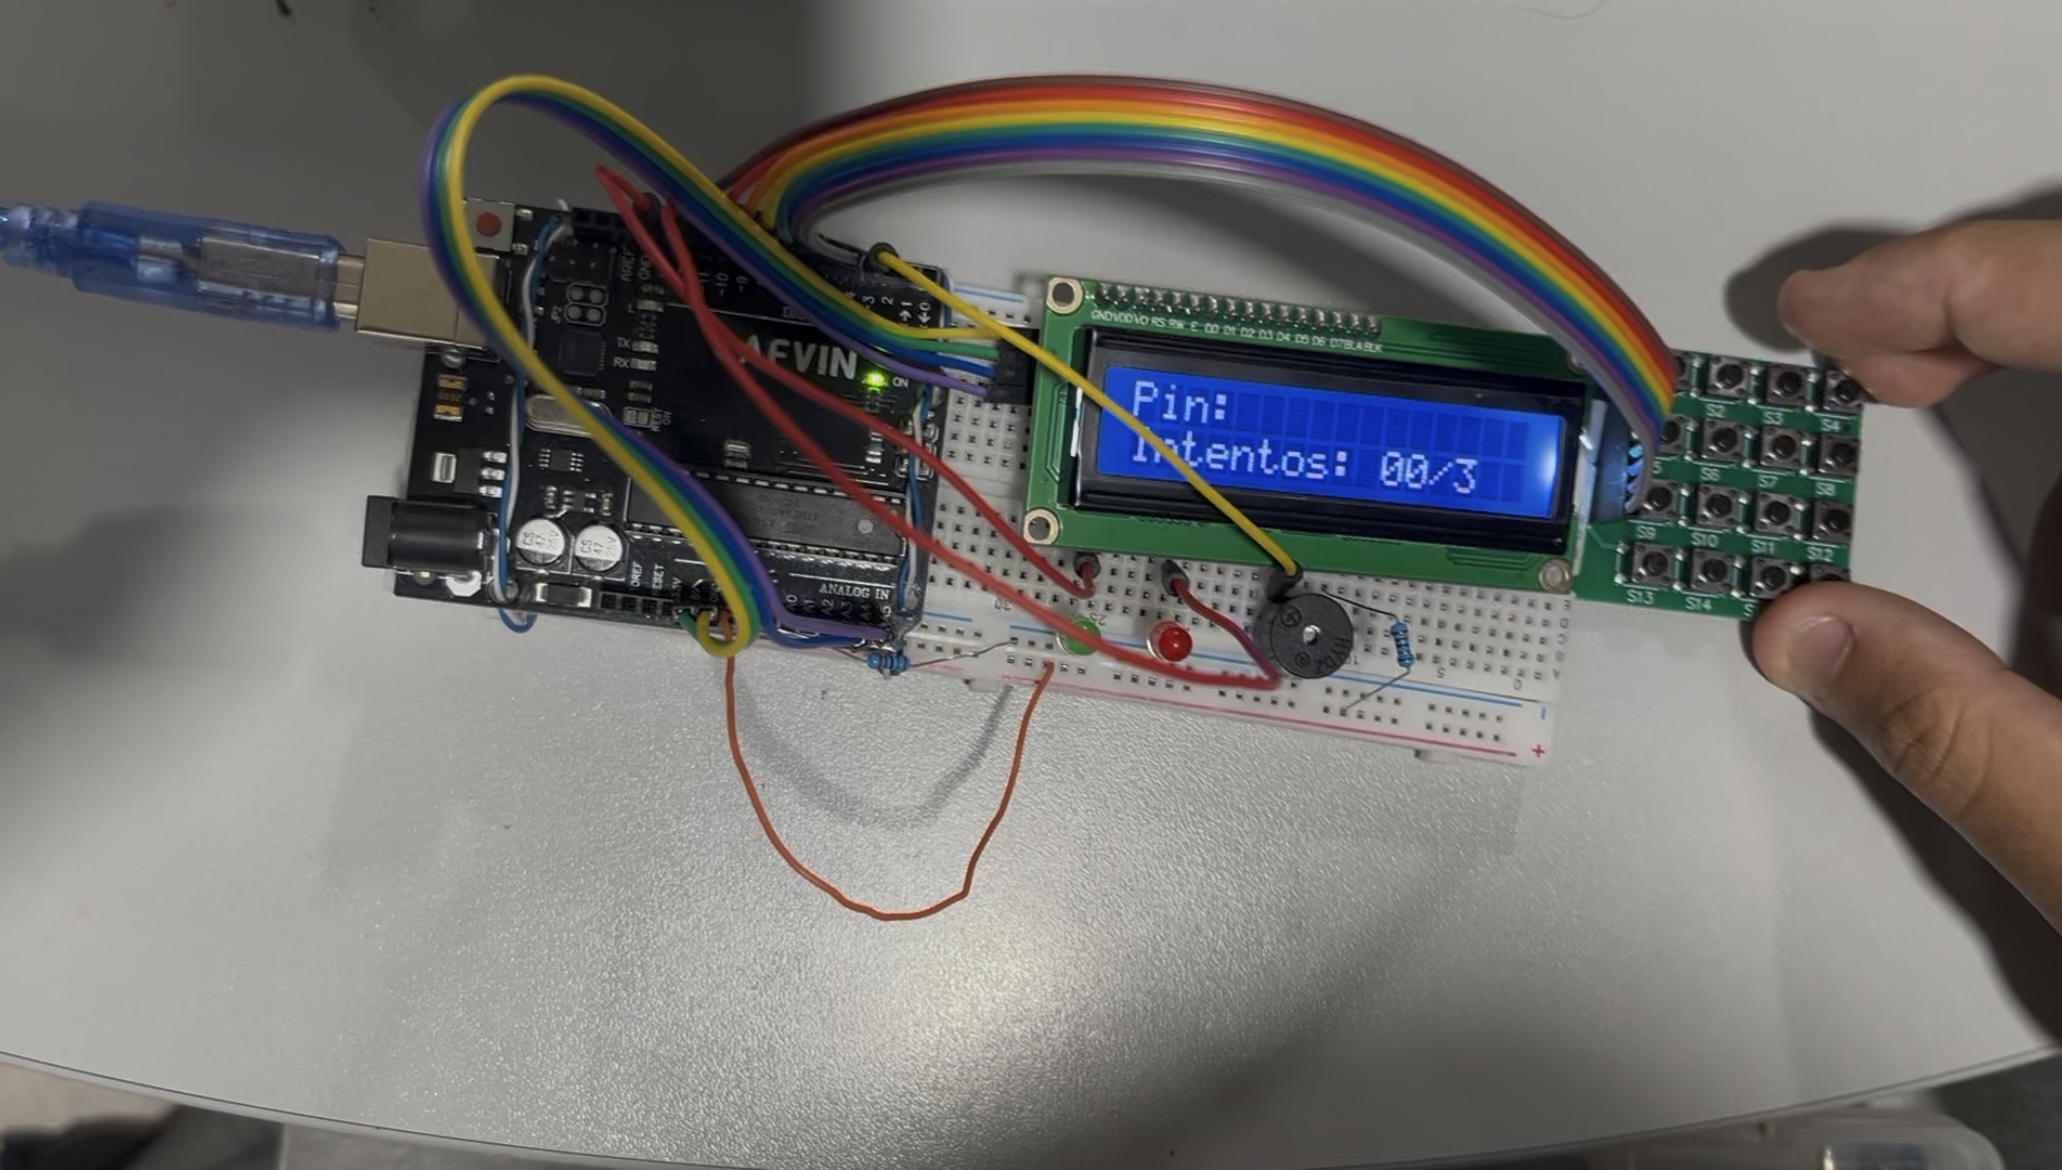
\includegraphics[width=0.8\columnwidth]{Anexos/Cerradura_Inicializada.png}
    \caption{Montaje general de la cerradura electrónica con LCD iniciado mostrando el mensaje \texttt{Pin:}, teclado 4×4, LEDs y buzzer. Fuente: elaboración propia.}
    \label{fig:cerradura_inicio}
\end{figure}

El diagrama de conexión completo se presenta en la sección de anexos correspondiente (Figura~\ref{fig:Cerradura_electronica}).

\subsubsection{Procedimiento de programación}

El programa se estructuró de forma modular, agrupando las funciones según su propósito:
\begin{itemize}
    \item \textbf{Módulo de LCD e interfaz I\textsuperscript{2}C:} funciones de inicialización, escritura de comandos, envío de datos y posicionamiento del cursor, 
    implementadas mediante rutinas básicas de TWI.
    \item \textbf{Módulo del teclado matricial:} lectura por escaneo de filas, detección de pulsaciones y conversión a caracteres mediante un mapa interno. 
    Se emplearon retardos cortos de estabilización para eliminar rebotes mecánicos.
    \item \textbf{Módulo de EEPROM:} almacenamiento del PIN en memoria no volátil, con verificación de validez al inicio 
    e inicialización con valor por defecto (“1234”) en caso de no existir un PIN previo.
    \item \textbf{Módulo de retroalimentación:} control del LED verde, LED rojo y buzzer para representar estados del sistema 
    (acceso concedido, error, bloqueo, confirmación de cambio de clave, etc.).
\end{itemize}

\subsubsection{Flujo de operación}

El sistema inicia verificando la existencia de un PIN válido en la memoria EEPROM. 
Si no se detecta, se crea uno por defecto y se muestra el mensaje “Pin: ” en el LCD.  
A partir de allí, el usuario puede:
\begin{enumerate}
    \item Ingresar el PIN y confirmar con la tecla \texttt{A}.  
    \item Iniciar el cambio de contraseña con la tecla \texttt{C}.  
    \item Borrar el ingreso actual con la tecla \texttt{B}.  
    \item Utilizar la tecla \texttt{D} como llave maestra para desbloquear el sistema.
\end{enumerate}

Si el PIN ingresado tiene menos de 4 dígitos, el sistema muestra “Min 4 dígitos” y emite un pitido corto.  
Si el PIN es incorrecto, se incrementa un contador de intentos y se activa una señal acústica junto al LED rojo durante 500~ms.  
Tras tres intentos erróneos consecutivos, el sistema entra en modo de bloqueo, 
activando una alarma visual y sonora que permanece encendida hasta que se ingrese la tecla maestra \texttt{D}.  
Cuando el PIN es correcto, se activa el LED verde y el buzzer emite tres pulsos cortos de confirmación.

El modo de cambio de PIN consta de tres fases secuenciales: verificación del PIN actual, ingreso del nuevo PIN (4–6 dígitos) y confirmación.  
El nuevo valor se almacena en la EEPROM mediante escritura byte a byte.

\subsubsection{Validación funcional}

Las pruebas de verificación se realizaron en hardware real, 
evaluando la respuesta del sistema ante diferentes secuencias de entrada: 
PIN correcto, PIN incorrecto, longitud insuficiente, cambio de clave y condición de bloqueo.  
En cada caso, se registraron los mensajes mostrados en el LCD y los patrones de activación del buzzer y LEDs, 
confirmando el cumplimiento del comportamiento esperado definido en el diseño lógico.
